\usepackage{booktabs}
\usepackage{empheq}
\setcounter{secnumdepth}{2}
\usepackage{amsmath}

\usepackage{color}

\usepackage{mdframed}
\usepackage{xcolor}
\definecolor{lightgray}{gray}{0.98}

% Custom environment for background box
\newmdenv[
  backgroundcolor=lightgray,
  skipabove=10pt,
  skipbelow=10pt,
  leftmargin=0,
  rightmargin=0,
  innerleftmargin=10pt,
  innerrightmargin=10pt,
  innertopmargin=10pt,
  innerbottommargin=10pt
]{graybox}

% \newenvironment{graybox}{
%   \definecolor{shadecolor}{rgb}{0.9, 0.9, 0.9}  % gray
%   \color{white}
%   \begin{shaded}}
%  {\end{shaded}}
 


\usepackage{framed}
\setlength{\fboxsep}{.8em}

\newenvironment{blackbox}{
  \definecolor{shadecolor}{rgb}{0, 0, 0}  % black
  \color{white}
  \begin{shaded}}
 {\end{shaded}}
 
% \newenvironment{greybox}{
%   \definecolor{shadecolor}{rgb}{0.9, 0.9, 0.9}  % light grey??
%   \color{white}
%   \begin{shaded}}
%  {\end{shaded}}
 
% \usepackage[left=1in,top=1in,right=1in,bottom=1in]{geometry}

\usepackage{caption}
\captionsetup[figureNoLabel]{labelformat=empty, justification=raggedright}

%\usepackage{wrapfig}

\usepackage{amsfonts}
\usepackage{amsmath}
\usepackage{amssymb}
\usepackage{verbatim}
\usepackage{fancyvrb}
\usepackage{framed}
\usepackage{xcolor,colortbl}
\usepackage{setspace}
\usepackage{scalefnt}
\usepackage{array}
\usepackage{color}
\usepackage{xcolor}
\usepackage{xr}
\usepackage{tabularx}
\usepackage{caption}
\usepackage{multirow}
\usepackage{graphicx}

\setlength{\fboxsep}{.8em}

\renewcommand{\hrulefill}{%
  \leavevmode\leaders\hrule height 2pt\hfill\kern0pt }
  
\renewcommand{\dotfill}{%
  \leavevmode\cleaders\hbox to 0.60em{\hss .\hss }\hfill\kern0pt }
  
\usepackage{pdfpages}
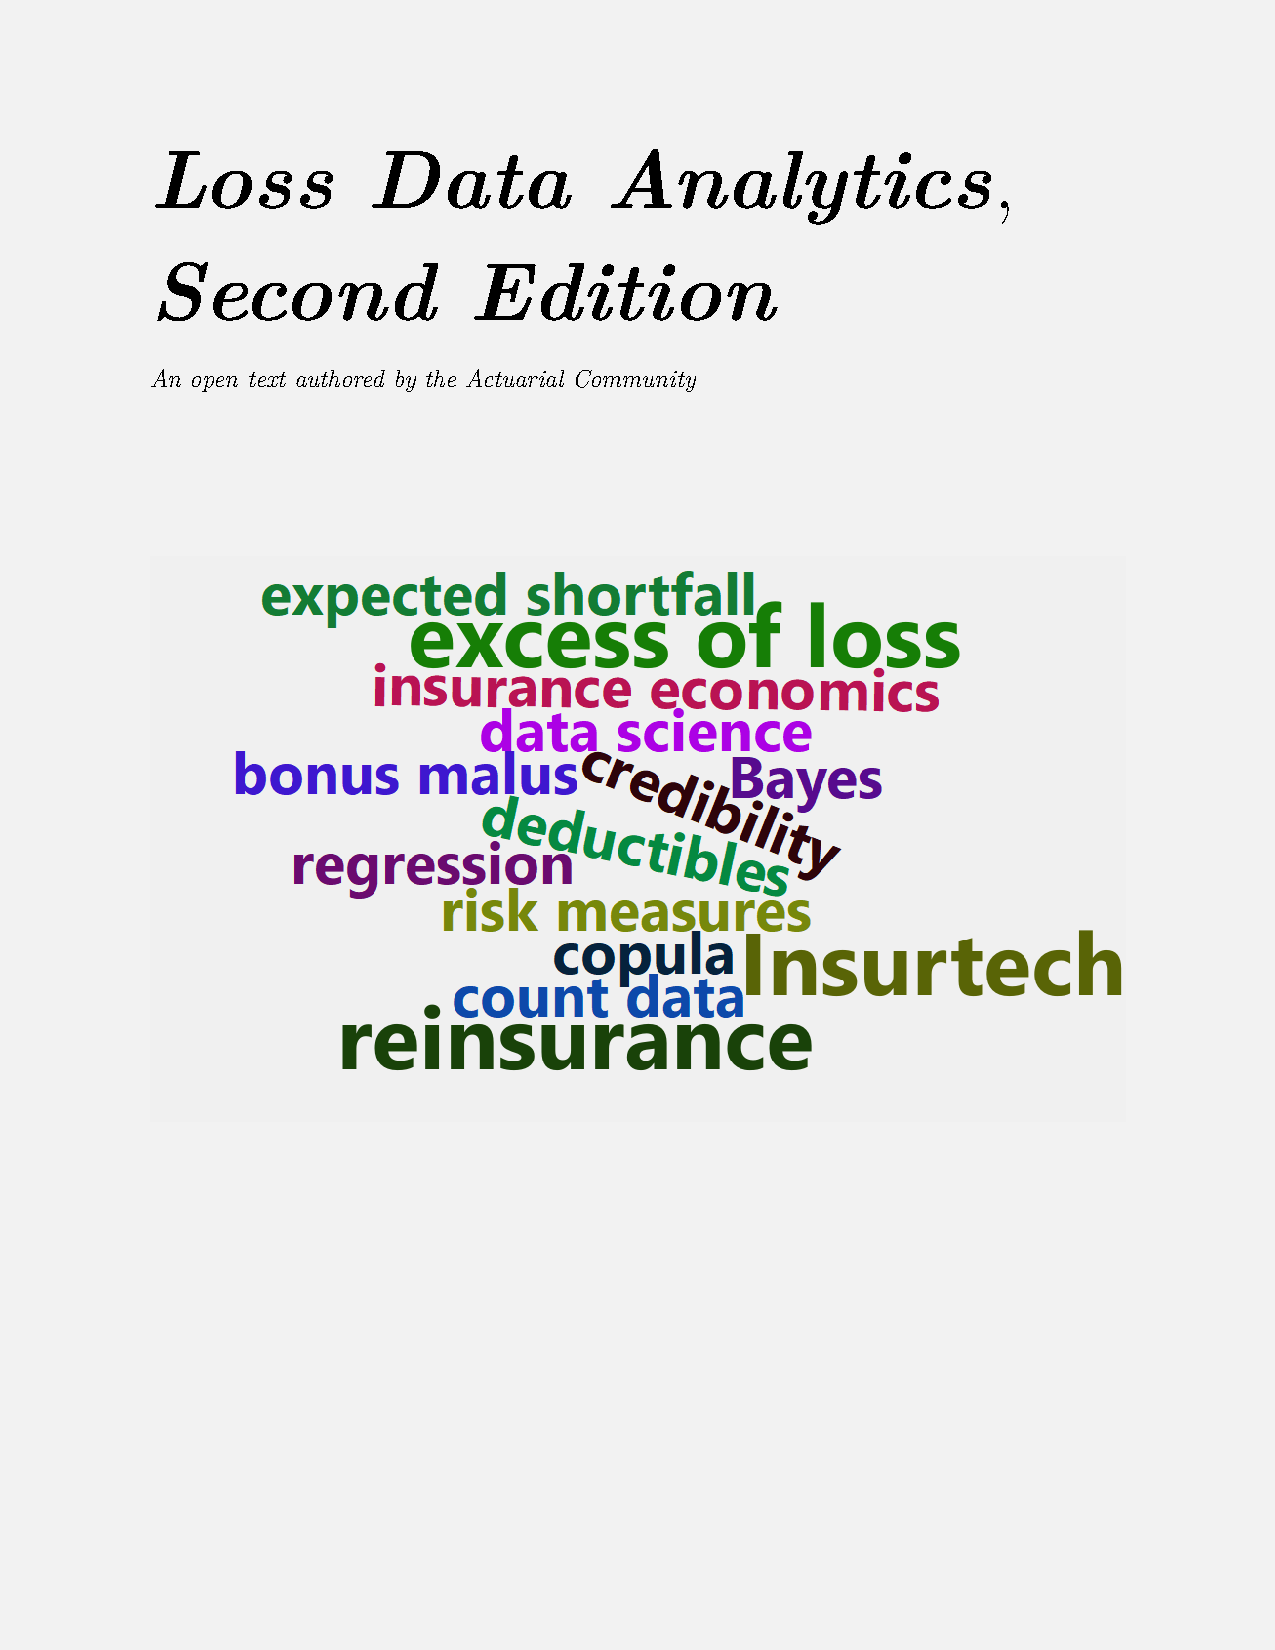
\includepdf{"Figures/FreesCoverIdea19Sept2024.pdf"}

\usepackage{makeidx}
\makeindex

